% ============================================================
% v2/sections/results.tex  結果（短縮・再構成版 2026-10-27）
% 数字は sections/results.tex（第2弾の照合済み）と Claude Code の報告（A・B・C）から。
% 組1=s0，組2=s1，組3=s2（本番），組4=s3，組5=s4，組6=s5。
% ============================================================
\section{結果}\label{sec:results}

\begin{figure}[tbp]
  \centering
  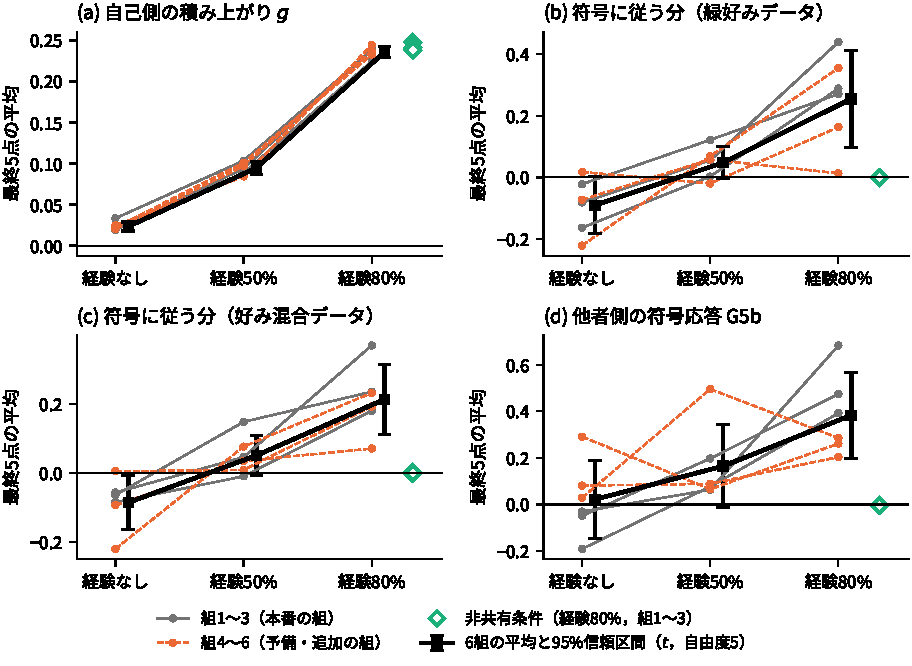
\includegraphics[width=\linewidth]{figs/central}
  % 元：paper/figs/central.pdf（G3，符号に従う分（緑好み・好み混合），G5b。6組，非共有は白い菱形）
  \caption{自分側の見込みと他者側への転用．横軸は経験の量．細い線は各組（組1〜3 は灰の実線，組4 は橙の破線，組5・6 は橙の点線と白抜きの四角），太い線は6組の平均と95\%信頼区間，白い菱形は非共有条件（組1〜3）．(a) 自分側の積み上がり $g$（事前登録）．(b)(c) 他者側の符号に従う分（緑好みデータ，好み混合データ．組1〜4 では事後に定義）．(d) 他者側の符号応答 G5b（事前登録）．}
  \label{fig:central}
\end{figure}

\begin{table}[tbp]
  \centering
  \footnotesize
  \setlength{\tabcolsep}{4pt}
  \caption{組をまたいだ主な差（全6組．各組の最終5点の平均を1つの値とし，組どうしを対にした差の平均と $t$ の95\%信頼区間．事前登録外の記述）}
  \label{tab:summary}
  \begin{tabular}{llll}
    \toprule
    指標 & 50\% $-$ 経験なし & 80\% $-$ 50\% & 80\% $-$ 経験なし \\
    \midrule
    自分側の積み上がり $g$ & $+0.071$ [$+0.064$, $+0.079$] & $+0.141$ [$+0.131$, $+0.152$] & $+0.213$ [$+0.205$, $+0.221$] \\
    G5b & $+0.143$ [$-0.109$, $+0.394$] & $+0.218$ [$-0.066$, $+0.503$] & $+0.361$ [$+0.057$, $+0.665$] \\
    符号に従う分（緑好み） & $+0.138$ [$+0.028$, $+0.248$] & $+0.207$ [$+0.050$, $+0.363$] & $+0.345$ [$+0.132$, $+0.557$] \\
    符号に従う分（好み混合） & $+0.137$ [$+0.027$, $+0.246$] & $+0.163$ [$+0.059$, $+0.267$] & $+0.300$ [$+0.174$, $+0.425$] \\
    \bottomrule
  \end{tabular}
  % 出典：v13 まとめ §11（第2弾の照合済み）。組ごとの値は補足資料の表。
\end{table}

\subsection{自分側の見込み}\label{sec:res-self}
自分側の積み上がり $g$ は経験の量に応じて段階的に大きくなった（図\ref{fig:central}(a)，表\ref{tab:summary}）．
本番の3組の値は，経験なし条件で $+0.019$〜$+0.033$，経験50\%条件で $+0.089$〜$+0.103$，経験80\%条件で $+0.225$〜$+0.240$ であった．
事前登録した組ごとの判定では，経験なし条件との差は経験50\%条件・経験80\%条件とも6組すべてで成り立ち，経験80\%条件が経験50\%条件を上回ることも6組すべてで成り立った．
経験なし条件の $g$ も小さく正であり，見込みは経験なし条件よりはっきり強く生まれた，と言うのが正確である．

前提とした自己位置の追跡（運動が見えるステップで $h^1$ から A-1 の位置を読む決定係数 0.80 以上）は，経験50\%条件では6組とも満たしたが，経験80\%条件では6組とも満たさなかった（0.70〜0.75）．
自分の学習データと同じ作りのテストでは 0.99 であり，赤の角にとどまる学習データによる，経験していない場面への一般化の弱さと考えられる．
$g$ などの指標は位置の読み出しを使わずモデル自身の予測から測るので計算はできるが，経験80\%条件の値はこの状態を含むものとして読む必要がある．
前提を満たした経験50\%条件と経験なし条件の比較だけでも，経験によって見込みが生まれることは6組で成り立つ．
非共有条件でも自分側の見込みは経験80\%条件と同じように生まれた（$g$ は $+0.238$〜$+0.248$）．

\subsection{他者側への転用}\label{sec:res-other}
process-2 の一つの範囲に $\pm a$ を入れると，経験80\%条件では予測の中の A-2 がその向きにずれた（図\ref{fig:central}(d)）．
本番の3組では，経験80\%条件の G5b は $+0.392$〜$+0.682$（経験なし条件 $-0.191$〜$-0.030$）で，事前登録した判定に3組とも合格した．
全6組では経験なし条件との差が5組で成り立ち，組をまたいだ差も0を含まなかった（表\ref{tab:summary}）．
自己位置の追跡の前提を満たした経験50\%条件でも，G5b は $+0.063$〜$+0.197$ で，事前登録した判定に合格した（本番の3組中2組）．
ただし組をまたいだ段階ごとの差は0を含み，G5b で組をまたいで示せるのは経験80\%条件が経験なし条件より大きいことまでである．
外れた組は，経験なし条件の G5b が大きかった組4（$+0.291$）と，経験50\%条件が経験80\%条件を上回った組6である（補足資料）．
A-2 の本当の快・不快を用いる符号に従う分では，二つのデータとも二つの段階の差が0を含まなかったが（表\ref{tab:summary}），この指標は組1〜4 では事後に定義したものである（\ref{sec:evaluation}節）．
これらは，自分側で学んだ傾向が他者側の予測に反映されること（転用）を示すが，他者の行動の予測が正確になることは示さない（\ref{sec:res-projection}節）．

非共有条件では他者側の働きは消えた（G5b は3組とも $-0.01$〜$+0.01$，符号に従う分も0前後）．
それでも $h^2$ から A-2 の位置を読む決定係数は 0.91〜0.93 で，他者の状態を追う力は育っていた．
他者の状態を追えることだけでは，他者側の価値に関わる働きは生じない．
ただしこの結果は，process-2 の快・不快の入口が学習されないという構成からほぼ予想されるものである．

\subsection{成立条件：価値の信号と行動の対応}\label{sec:res-signrand}

\begin{figure}[tbp]
  \centering
  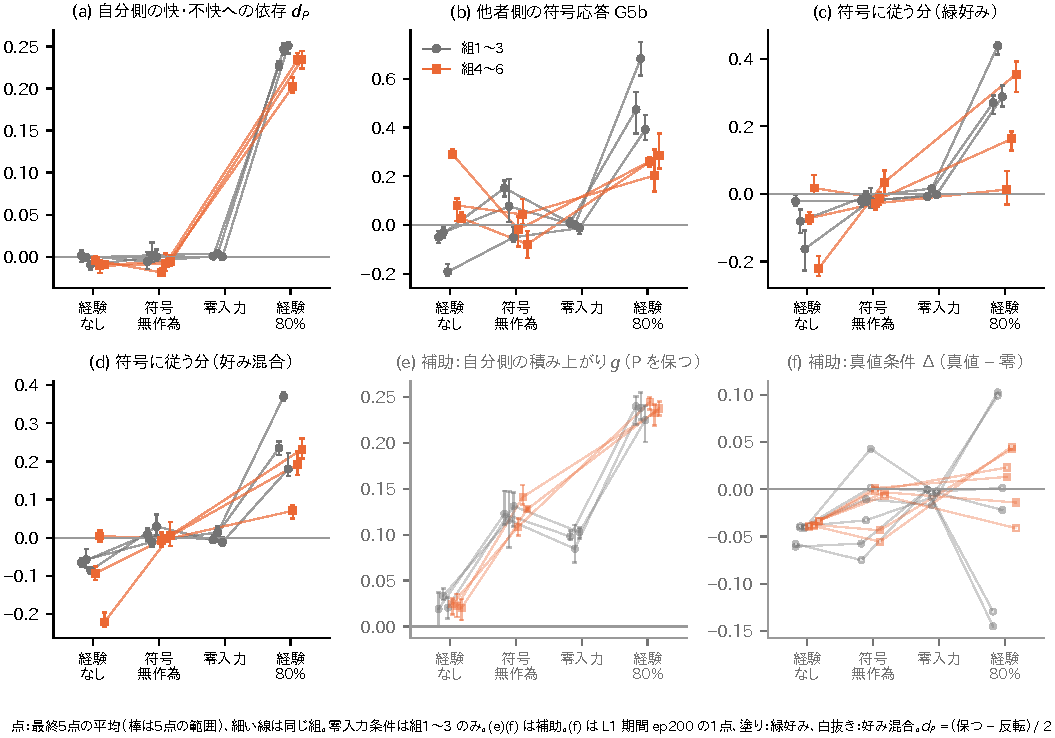
\includegraphics[width=\linewidth]{figs/c_signrand}
  % 元：paper/figs/c_signrand.pdf。パネルの順を (a) d_P，(b) G5b，(c)(d) 符号に従う分，(e) g，(f) Δ（補助，薄く）に
  %   並べ替えてもらう（第3弾の指示書）。零の条件が加わったら差し替え。
  \caption{位置の分布をそろえた対照（符号無作為条件）．横軸は経験なし条件，符号無作為条件，経験80\%条件．主な量は (a) 自分側の快・不快への依存 $d_P$，(b) 他者側の符号応答 G5b，(c)(d) 符号に従う分（緑好みデータ，好み混合データ）．(e) 快・不快を保ったときの自分側の積み上がり $g$ と (f) 真値条件の $\Delta$ は補助．組1〜3 を線で結ぶ．}
  \label{fig:signrand}
\end{figure}

経験80\%条件と同じ軌跡で快・不快の符号だけを無作為にすると，自分側の快・不快への依存と他者側の符号に従う分は0前後になり，他者側の符号応答 G5b も大きく弱まった（図\ref{fig:signrand}）．
自分側の $d_P$ は0前後（経験80\%条件 0.23〜0.25），符号に従う分は二つのデータとも $-0.02$〜$+0.03$（経験80\%条件 $+0.18$〜$+0.44$）であった．
G5b は組1〜3 で $+0.15$，$+0.08$，$-0.05$ と，3組とも経験80\%条件（$+0.47$，$+0.68$，$+0.39$）より小さかったが，3組とも経験なし条件（$-0.05$，$-0.03$，$-0.19$）よりは大きく，完全に消えたとは言えない．
事前登録した予想のうち，他者側の働きが経験80\%条件より小さくなること（G5b・符号に従う分）と自分側の快・不快への依存が小さくなること（$d_P$）は，3組とも成り立った．
照合の他者特徴基準の BA も 0.50〜0.57 にとどまった（経験80\%条件 0.74〜0.78）．
一方，次の視界の予測誤差と自己位置の追跡は経験80\%条件に近く（追跡の決定係数は【要確認】），学習も安定していた（学習の損失は約5\%高いだけ）．
自分側の予測の質を保ったまま，快・不快に関わる働きが大きく弱まったことになる．
ただし，快・不快を保ったときの $g$ は経験なし条件より $+0.05$〜$+0.13$ 大きく残った．
これは事前登録で注意として挙げた，快・不快によらず赤へ向かう癖に当たる．

この対照は，位置・運動・視界の系列をそろえたまま，価値の信号と行動の一貫した対応だけを壊したものである．
したがって，快・不快に従う自分側の見込みと，それが他者側に及ぶ働きは，学習データの位置の偏りだけでは説明できず，価値の信号と行動の一貫した対応に大きく依存すると言える．
一方で，赤へ近づくという行動の履歴そのものは変えていないので，価値に従って動いた経験のあらゆる効果を識別したものではない．
G5b に残った分は，赤への癖や，位置の手がかりとしての快・不快の大きさを含みうる．
快・不快を常に零にした条件の結果は【結果待ち】である．

\subsection{成立条件：自分の予測の力学の再利用}\label{sec:res-copy}
学習を終えた非共有条件のモデルに自分側の重みを写すと，視覚予測器を通らない量では，共有ありの経験80\%条件と同じ形の働きが戻った（事前登録外の確認を含む．詳細は補足資料）．
LSTM の重みをすべて写すと，照合の他者特徴基準の BA は 0.75〜0.77 になり（元の非共有条件 0.41〜0.49，経験80\%条件 0.74〜0.78），経験なし条件の非共有モデルに同じように写した場合（0.35〜0.52）との差は3組とも正で信頼区間は0を含まなかった（$+0.25$〜$+0.41$）．
真値条件の $\Delta$ でも，経験ありの重みを写したときにだけ，経験80\%条件と同じく A-2 の規則の確率による変化が現れた．
快・不快を受ける入口の8列だけを写した場合は，G5b は0前後のままで（$-0.035$〜$+0.030$，事前登録した予想は不支持），照合も戻らなかった（0.45〜0.55）．
他者側への価値に関わる傾向の転用は，快・不快の入口の重みだけでは説明できず，自分の経験で学習された LSTM のほかの重みや計算にも依存する可能性が示された．
ただし，すべて写す操作は再帰の結合だけでなく入力の重みやバイアスも同時に変えるので，どの重みが要るかは特定していない．
すべて写すと他者の追跡が基準を下回り（$h^2$ の決定係数 0.60〜0.75），予測画像を通る量（G5b，符号に従う分）は，写した $h^2$ と視覚予測器の食い違いのために判定できなかった．
学習中に重みを共有することと学習後に写すことが同等であるとも言えない．

\subsection{転用は他者の予測を正確にするか}\label{sec:res-projection}

\begin{figure}[tbp]
  \centering
  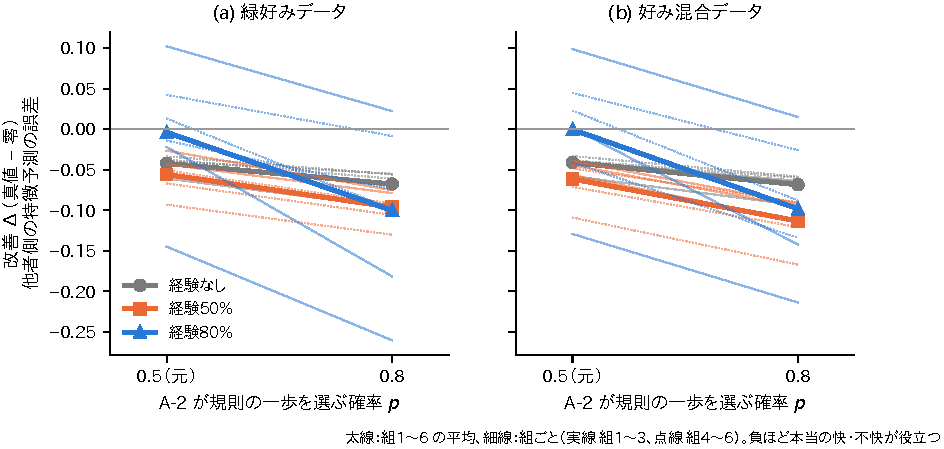
\includegraphics[width=\linewidth]{figs/a_cross_delta}
  % 元：paper/figs/a_cross_delta.pdf
  \caption{他者の規則の確率を変えたときの，本当の快・不快の役立ち方．縦軸は真値条件の誤差から零を入れた誤差を引いた値 $\Delta$（負なら役立つ）．横軸は A-2 が規則の一歩を選ぶ確率 $p$（実際に規則で動いた一歩は $p=0.5$ で約46〜47\%，$p=0.8$ で約57\%）．(a) 緑好みデータ，(b) 好み混合データ．細い線は各組（組1〜3 は実線，組4〜6 は点線），太い線は全6組の平均．}
  \label{fig:cross}
\end{figure}

転用が他者の行動の予測を正確にするかを，A-2 の本当の快・不快を process-2 に入れたときの他者側の特徴予測の誤差で調べた．
誤差は経験なし条件 0.25〜0.29，経験50\%条件 0.24〜0.28 に対し，経験80\%条件では 0.38〜0.42 と大きかった（段階IIを行った組1〜4，二つのデータ）．
経験なし条件と経験50\%条件の値はほぼ同じであり，経験による転用が予測を正確にしたことは示されなかった．
経験80\%条件で零を入れるより悪かったのは，緑好みデータで4組中2組，好み混合データで3組であった．
この悪化は予想していなかった結果である．

A-2 の規則の確率を 0.5 から 0.8 にすると，経験80\%条件では $\Delta$ が小さくなり（本当の快・不快がより役立ち），その変化は経験50\%条件・経験なし条件より大きかった（図\ref{fig:cross}）．
組をまたいだ変化は経験80\%条件で $-0.096$ [$-0.139$, $-0.054$]（緑好み），$-0.098$ [$-0.125$, $-0.071$]（好み混合），経験50\%条件との交互作用は $-0.056$ [$-0.100$, $-0.012$]，$-0.046$ [$-0.072$, $-0.020$] で，事前登録した三つの予想は両データで6組すべて成り立った．
ただし，A-2 の確率を上げるとどの条件でも本当の快・不快はいくらか役立つようになり，悪化は消えずに小さくなった組が多く，組2 では零より悪いままであった．
また，確率を上げると A-2 も好きな色の角への滞在が増え（後半で好きな色から距離5未満にいる割合 0.99〜1.00），位置の分布も同時に変わる．
自分と他者の確率が一致したときに最もよく役立つことも示していない．
符号無作為条件でも，経験80\%条件の $\Delta$ そのものが組によってそろわず（悪化がはっきりしていたのは組2 だけ），悪化の原因は判定できなかった．
したがって，この結果は，自他の行動の仕方の違いが本当の快・不快の役立ち方に影響する可能性を示すにとどまり，自分の行動の仕方を他者に当てはめる投影と断定はできない．

\subsection{他者の好みの表現と推定}\label{sec:res-pref}
他者用モジュールは，構成を4通りに変えても（自由出力，形の制限，A-2 を隠した学習，1ビット）他者の好みを書き出さなかった（補足資料）．
事前登録した主の構成（経験50\%条件）では，T2・T5 とも4組中1組でしか合格の形にならず，その値（T2 $+0.03$〜$+0.05$，T5 $+0.04$〜$+0.05$）は本当の快・不快を入れた値（T2 $+0.60$，T5 $+0.42$）の 1/10 ほどであった．
一方，生成した $Q2$ を入れると他者側の特徴予測の誤差は本当の快・不快を入れた場合よりずっと小さく（0.116〜0.159 対 0.241〜0.276），モジュールは予測に役立つ位置の情報を伝えていた．
出力を1ビットに絞っても，好みと方角が食い違うエピソードで出力が好みに従う割合は 0.30〜0.41（経験80\%条件）で，方角の側に寄った．
これはモジュールの出力についての結果であり，内部状態に好みの情報がないことを示すものではない．

好みの候補を入れ比べる照合は，経験80\%条件の本番の3組で偶然を上回り（自己視界基準の BA 0.553〜0.701，事前登録した判定で合格），経験50\%条件では上回らなかった．
しかし方角だけの基準の BA は 0.708 [0.653, 0.759] で，自己視界基準ではモデルとの差が6組とも負（$-0.089$ [$-0.140$, $-0.038$]），他者特徴基準でも組をまたいでわずかに上回るにとどまった（$+0.049$ [$+0.026$, $+0.072$]，組ごとにはっきり上回ったのは組4 だけ）．
好みと方角が食い違うエピソードで選択が好みに従う基準を満たしたのは，他者特徴基準で6組中4組，自己視界基準で2組で，両方を満たしたのは組2 だけであった．
共有された予測の仕組みは，与えた候補をある程度区別できるが，他者固有の好みを独立に推定できることまでは示されなかった．
